\onehalfspacing

\chapter{Introduction}
\label{chap:Introduction}

Biological cells are complex structures comprising of various biomolecules.
The internal structure of the cell contains various membrane-bound organelles such as the nucleus, the ER (endoplasmic reticulum) and Golgi apparatus scattered throughout the cytoplasm.
\figref{fig:basic_image} shows the typically crowded intracellular environment with various organelles of diverse sizes.
\begin{figure}[tb]
\centering
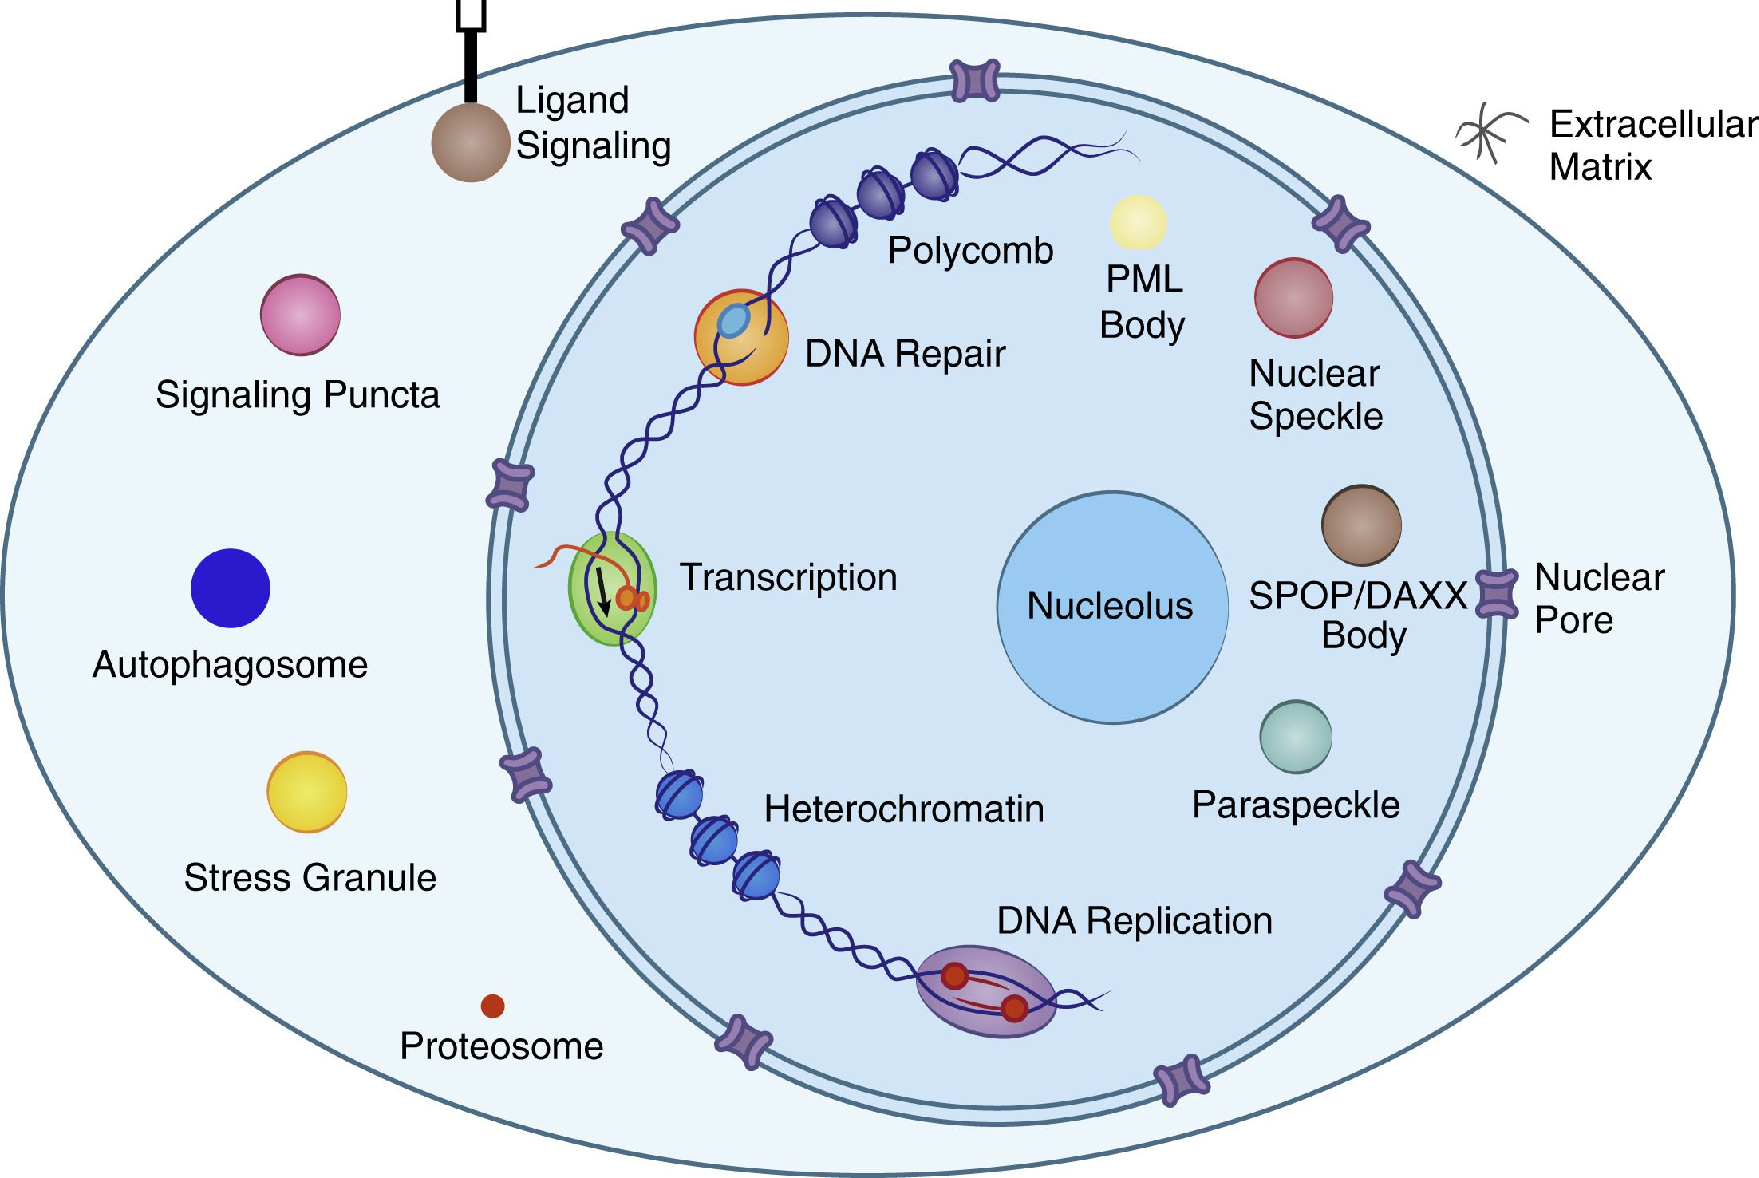
\includegraphics[scale=0.4]{MainContent/BioFigures/basic_image.pdf}
\caption{\textbf{Schematic showing the complex intracellular environment of the cell.}
Figure shows various membrane-bound and membrane-less organelles scattered throughout the cytoplasm inside the cell.
Reprinted with permission from Boija et al. \cite{Boija2021} under License number 5287881024090.
}
\label{fig:basic_image}
\end{figure}
For fulfilling it's many functions, the cell needs to spatially and temporally organize it's interior, consisting of macromolecules such as DNA and RNA, in an energetically efficient and fast manner.
This is an incredibly difficult task, as every second, thousands of biomolecular reactions happen inside the cell; see Ref. \cite{Flamholz2014}, of which a large fraction happens in aqueous mediums, see Ref. \cite{Mitrea2016}.

One way this is achieved is through utilizing membrane-bound organelles; see \figref{fig:basic_image}, which provide a physical barrier and act as a `sieve' for proteins and macromolecules entering from the intracellular environment.
For example, the ER and Golgi apparatus efficiently promote protein sorting and Mitochondria provide energy in form of ATP.
However, with the onset of advanced imaging technologies such as the Electron Microscope and techniques such as light microscopy, it has became clear that the intracellular environment also contains membrane-less organelles, also known as biomolecular condensates. 

\section{Biomolecular condensates}

In the last decade, much attention has been devoted to the formation of these aggregates.
The key reason for their formation is believed to be Liquid-liquid phase separation; see Refs. \cite{FloryBook,Keating2021}, which is the phenomena where molecules possessing certain physical or chemical properties aggregate (consisting of various proteins and macromolecules) and phase separate from the rest of the intracellular environment, similar to polymer condensation; see Ref. \cite{Hyman2014}.
For example, membrane-less organelles (or condensates) called P granules were observed in early stage \textit{C. elegans} worm embryos by Brangwynne et al. \cite{Brangwynne2009}, which played a key role in establishing the anterior-posterior axis for the embryos.
% \begin{figure}[t]
% \centering
% \includegraphics[scale=0.53]{MainContent/BioFigures/history.pdf}
% \caption{\textbf{Timeline of development of Liquid-liquid phase separation in biological cells}.
% Figure shows relevant milestones in the development of Liquid-liquid phase separation in the context of biological cells
% Image taken from Wang et al. \cite{Wang2021}.
% }
% \label{fig:history}
% \end{figure}
These condensates are diverse in their appearances and shapes; see \figref{fig:condensates_diverse}, possess complexity in their composition, have multi-layered structures and can have sizes ranging from nanometers; see Ref. \cite{Sabari2018}, upto micrometers; see Ref. \cite{Feric2013}.
\begin{figure}[tb]
\centering
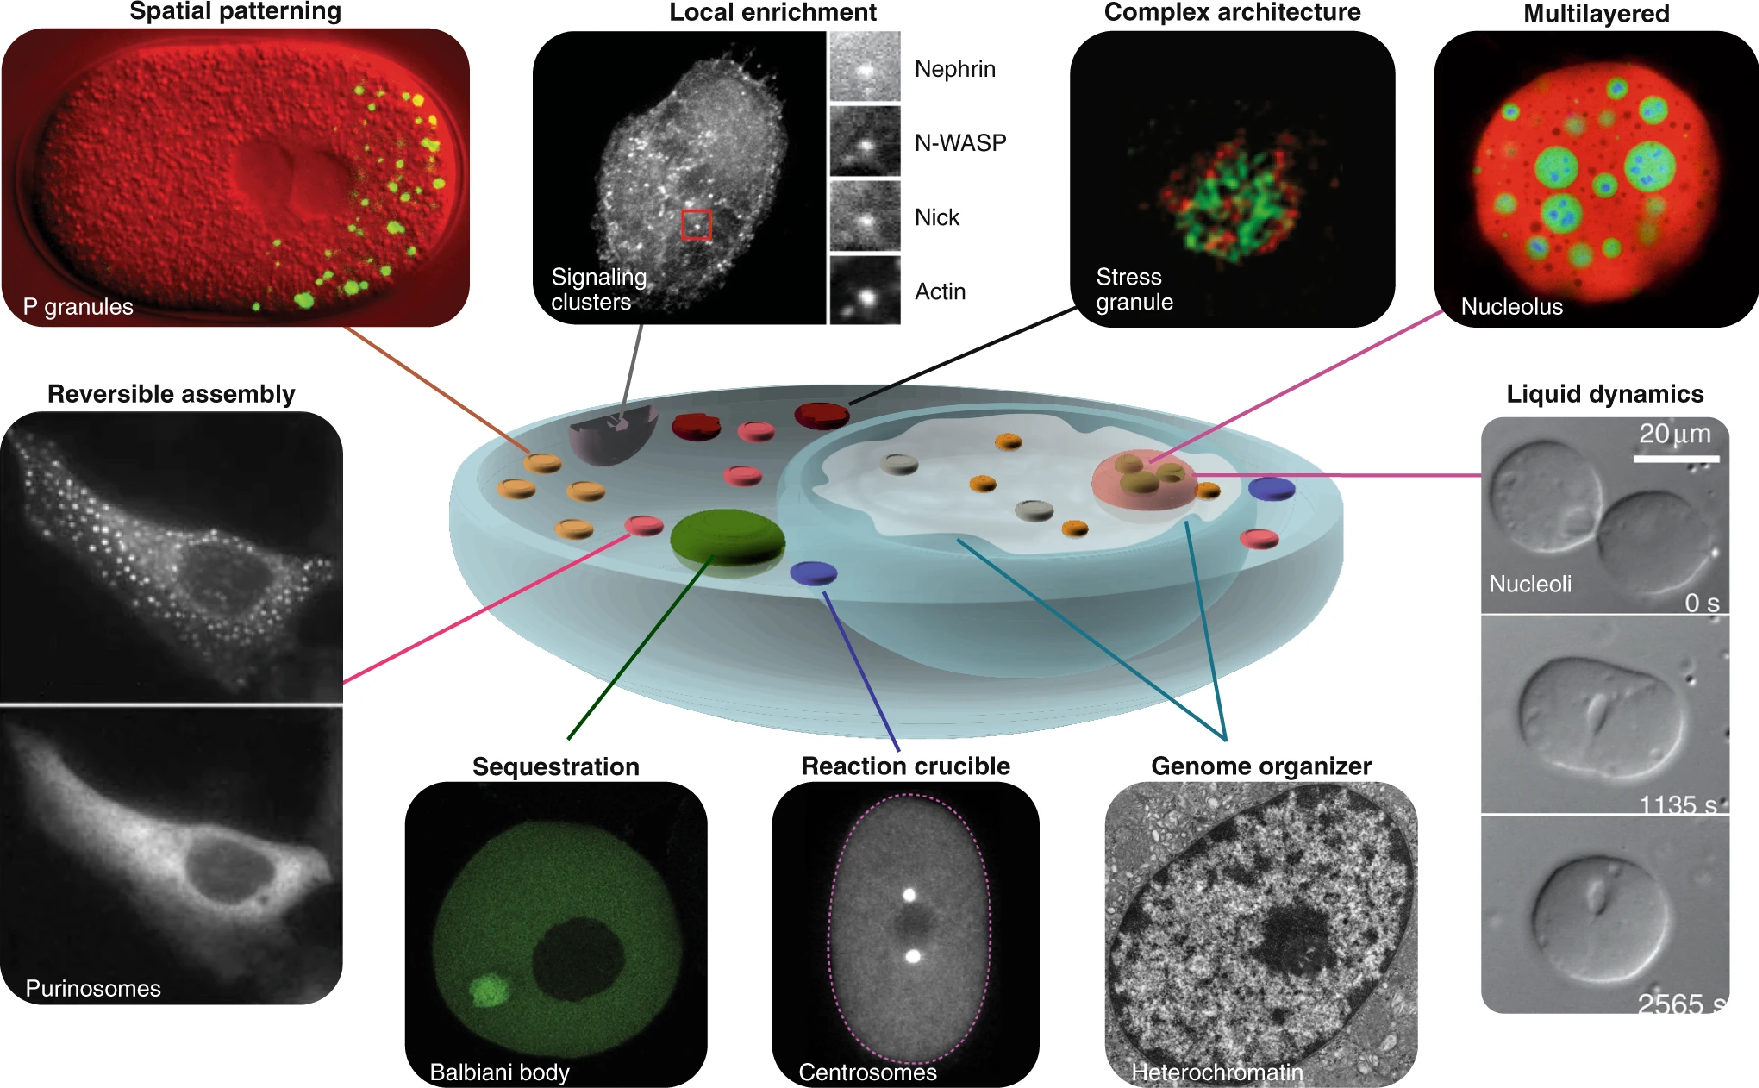
\includegraphics[scale=0.52]{MainContent/BioFigures/condensates_in_cells.pdf}
\caption{\textbf{Membrane-less organelles appear in diverse forms inside the cell.}
Membrane-less organelles (or condensates) possess diverse forms inside the cell and fulfil various functions, as seen from the schematic of the cell in the centre.
Reprinted with permission from Bracha et al. \cite{Bracha2019} under License number 5287590488572.
}
\label{fig:condensates_diverse}
\end{figure}

\section{Condensates are often liquid-like droplets}

Since these condensates form via Liquid-liquid phase separation, these condensates often possess qualities similar to liquid droplets; see \figref{fig:liquid_droplet}.
For example, it was shown by Brangwynne et al. \cite{Brangwynne2009} and Kroschwald et al. \cite{Kroschwald2015} that condensates: are spherical in shape, exhibit coalescence events, fuse with other condensates and form spherical droplets, deform and flow when encountering physical obstacles and regain their shape upon removal of the barrier.
Additionally condensates exchange material with the surroundings via diffusion; see Ref. \cite{Hubatsch2021}, and exhibit wetting phenomena as well; see Ref. \cite{Setru2021}.

\begin{figure}[tb]
\centering
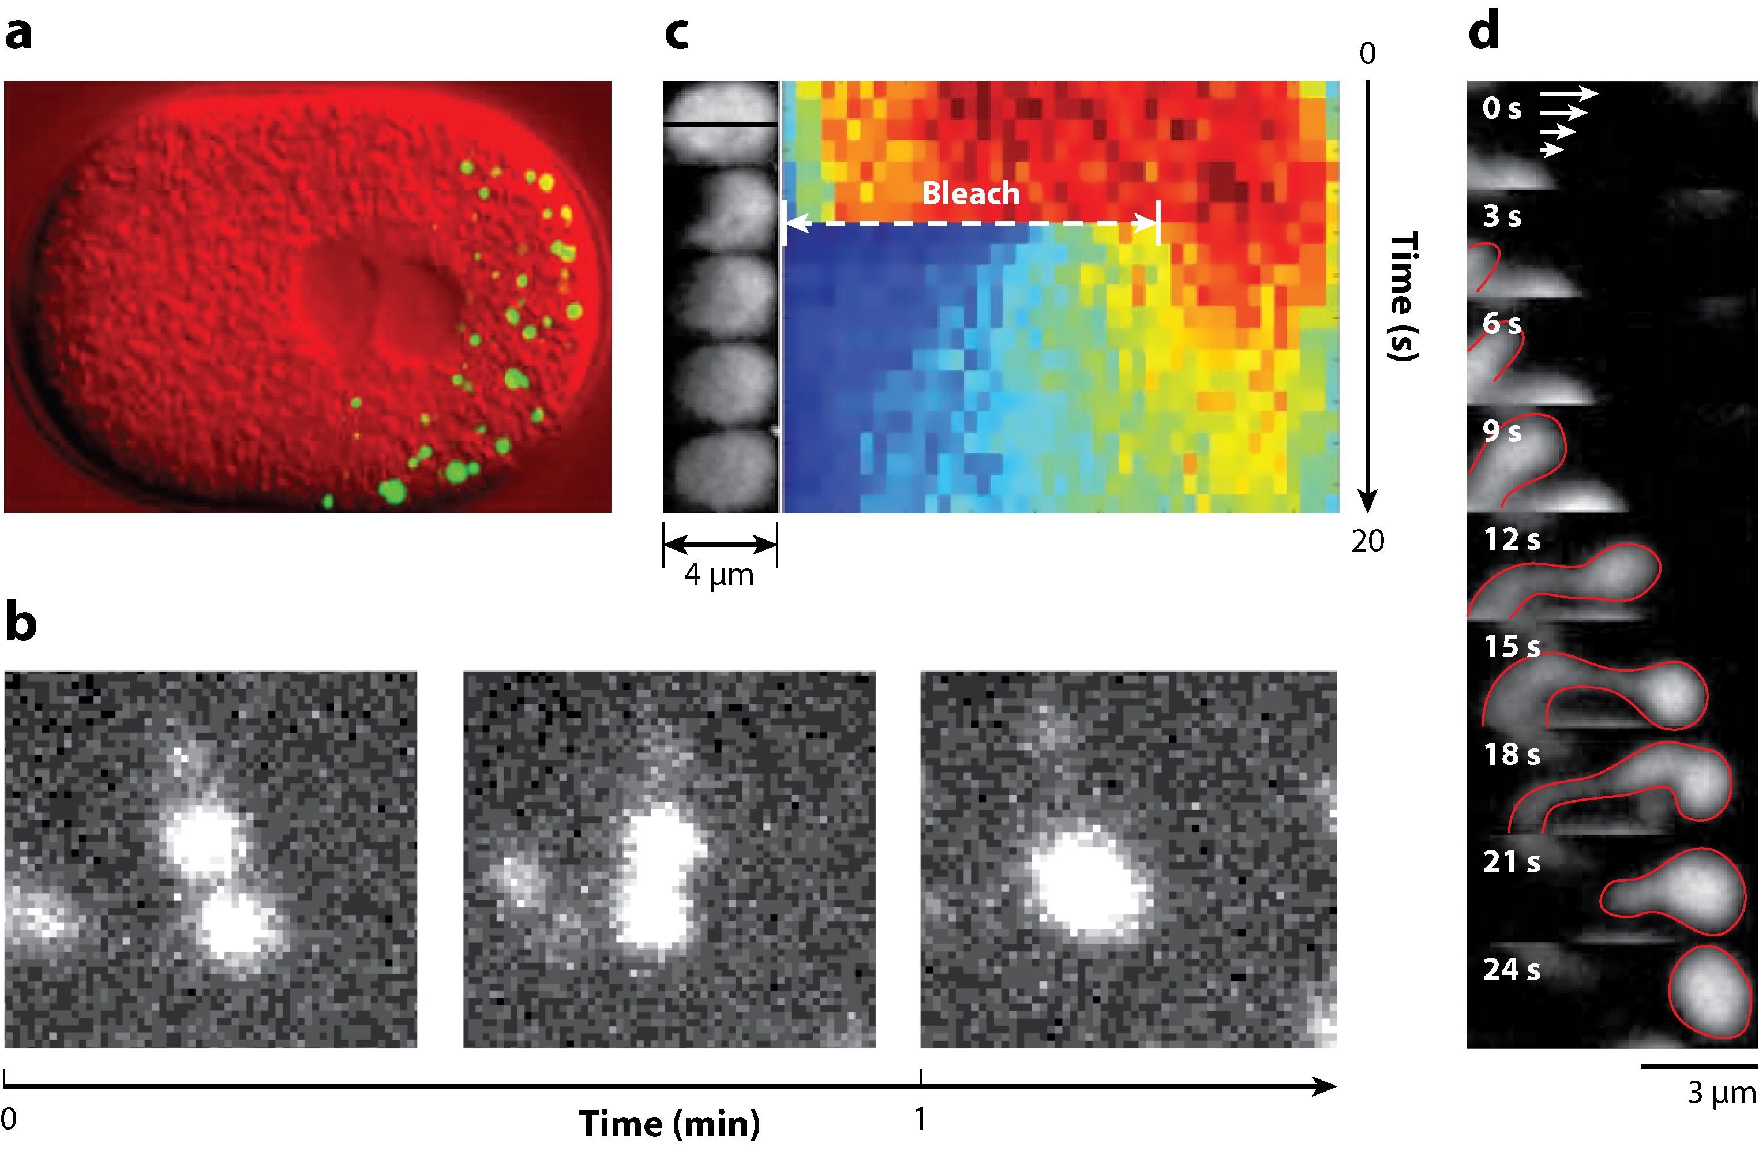
\includegraphics[scale=0.5]{MainContent/BioFigures/liquid_droplet.pdf}
\caption{\textbf{P granules are liquid droplets inside \textit{C.elegans} embryos}
(A) P granules localize to the posterior side of the early stage \textit{C.elegans} embryo.
(B) Two P granules fuse and assume a spherical shape, similar to liquid droplets in minutes.
(C) Photobleaching of half a P granule shows fluorescence recovery in seconds along with kymograph of linear intensity along the black line with red and blue indicating high and background intensity respectively. 
(D) P granules deform in shear flow.
Reprinted from Hyman et al. \cite{Hyman2014} and slightly modified with permission from the publisher with License number 1210872-1.}
\label{fig:liquid_droplet}
\end{figure}

However, not all condensates are liquid-like droplets.
Their structures and architectures can also differ, from being purely liquid-like to gel-like aggregates; see \figref{fig:architecture}.
In particular, condensates can have a liquid or solid shell enclosing a liquid core; see \figref{fig:architecture}A, see \figref{fig:architecture}B and see \figref{fig:architecture}C.
Examples of such condensates can be found in Refs. \cite{JAIN2016487,Putnam2019}.
Condensates can also form `nested droplets'; see \figref{fig:architecture}F, where nucleolus forms such an architecture; see Ref. \cite{Feric2013}.
Each of the sub droplets show liquid-like characteristics and are immiscible as a result of different viscosities. 
Although not common, condensates can also be non-spherical and form a network like assembly; see Ref. \cite{MA20181492} and \figref{fig:architecture}G.
They can even transition from a liquid droplet to a gel-like entity; see Ref. \cite{BOKE2016637} and \figref{fig:architecture}H, and can exhibit viscoelastic properties as well; see Ref. \cite{Jawerth2018}.
\begin{figure}[tb]
\centering
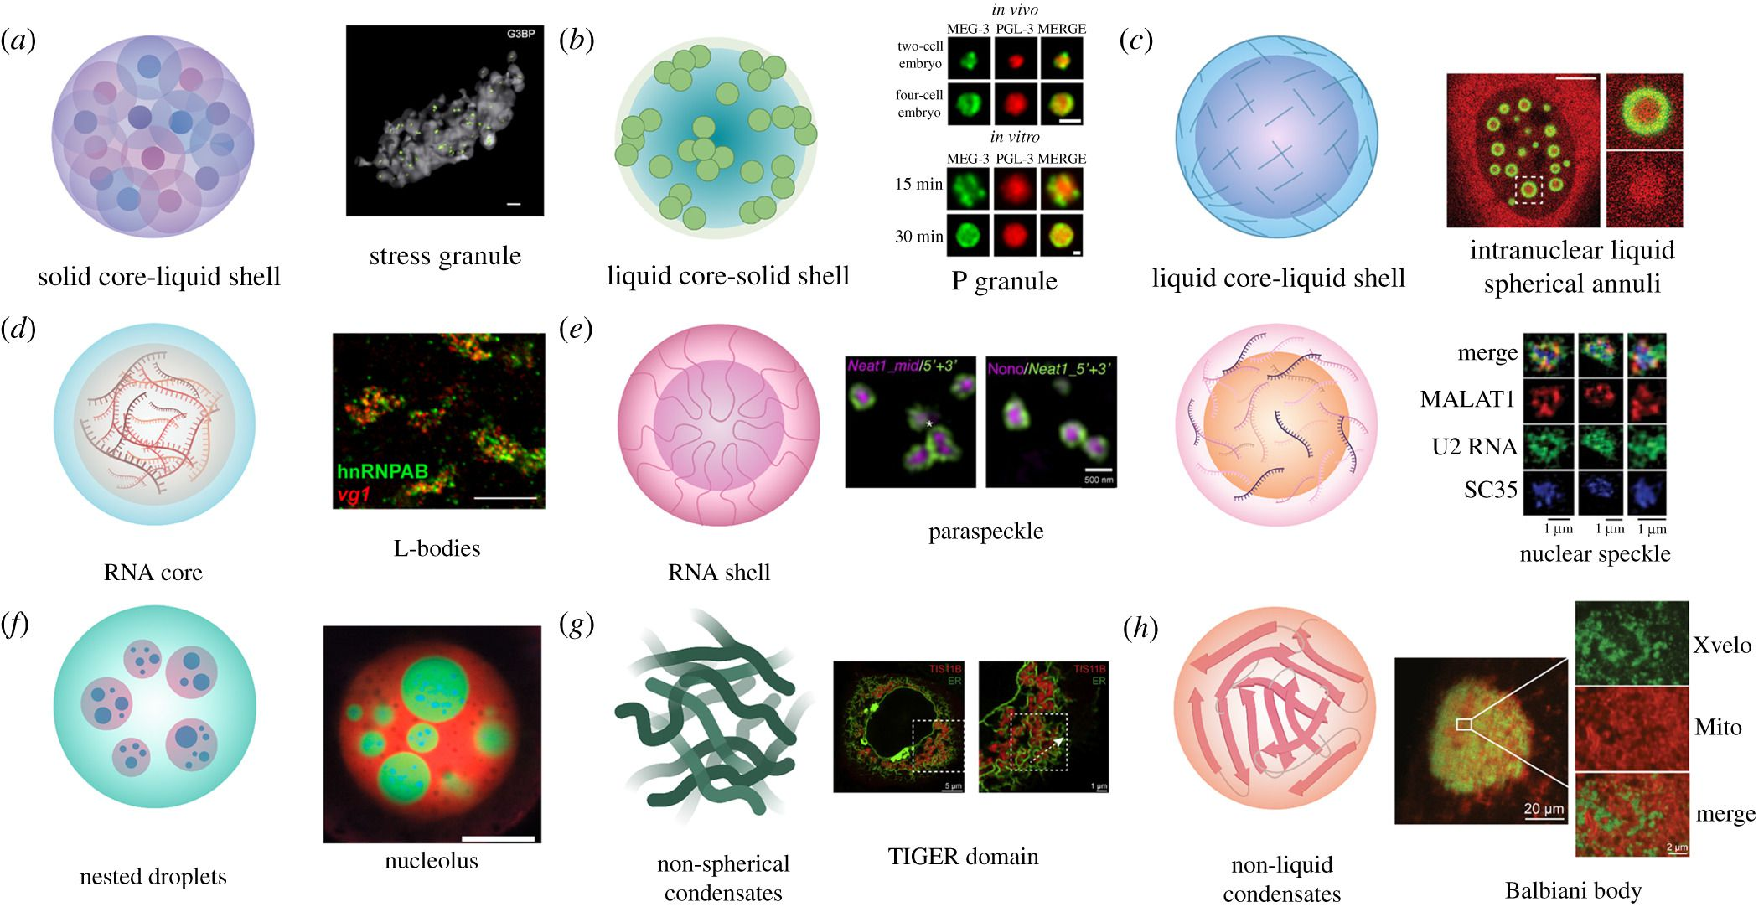
\includegraphics[scale=0.53]{MainContent/BioFigures/architecture.pdf}
\caption{\textbf{Collection of a few condensate architectures.}
Figure depicts collection of diverse architectures for biomolecular condensates ranging from liquid like droplets to gel-like structures. 
Reprinted with permission from Fare et al. \cite{Fare2021} under the Creative Commons Attribution License.
}
\label{fig:architecture}
\end{figure}
Having discussed the diverse architecture possible for condensates, we next discuss the important question: what purpose do they serve?

\section{Condensate function}

Biomolecular condensates have been found to be essential for a wide range of functions, a few being: rearranging molecules to facilitate RNA metabolism and stress signalling, but their precise role is still not well understood.
These functions exist across a wide range of length-scales as well: from molecular scale (for example, augmentation or suppression of chemical reaction rates, controlling folding dynamics of proteins) to the scale of the cell itself (for example, recruiting proteins to specific locations).
We discuss these functions from the context of length-scales.

\subsection{Functions on a molecular scale}

On the molecular scale, condensate formation can: a) Augment or inhibit reaction rates simply as a consequence of increased concentration of the reactants inside; see Refs. \cite{ANDERSSON2008275,Mingjian2018}, and b) Offer reaction specificity by selectively enhancing the functioning of certain biomolecules; see Ref. \cite{Peeples2020}.
Subsequently, condensates can alter local reaction rates and concentration of certain molecules.
They also play a role in regulating nucleation-dependant processes as well, which is evident in the accelerated nucleation of microtubules; see Refs. \cite{Huang2017,King2020}.

On the other hand, condensates can aid in suppression of reactions and decrease overall activity, which is achieved by isolating certain molecules from their regions of interactions or activity; see Refs. \cite{Hirose2014,POWERS2019177}.
Additionally, condensates like the nucleolus are thought to play a key role in prevention of misfolded protein aggregates when the cell encounters a sudden stress event.
Upon heat shock, certain thermally unstable proteins (which are prone to aggregation upon stress) are known to migrate in the nucleolus (so they do not aggregate), and are released back after the shock subsides; see Ref. \cite{Frottin2019}.

\subsection{Functions on the cellular scale}

On the cellular scale, condensates can recruit and concentrate cellular materials to distinct locations within the cell.
Consequently, size presents a big hurdle for the cell to compartmentalize it's interior and a clear correlation has been observed with cell size and aberrant condensate formation.
One way the cell alleviates this problem is by forming different condensates and optimizing their functions accordingly; see Refs. \cite{LEE2013572,Lee2015}, thus exhibiting the importance of spatiotemporal regulation of condensates by the cell.

However, large cells such as neurons, oocytes and muscle cells still must spend additional energy to spatially organize their interior, as compared to smaller cells.
In particular, transport of RNA-protein condensates in neurons is essential for neuron functioning; see Refs. \cite{LIAO2019147,KANAI2004513}.
These condensates are utilized to transport mRNA molecules efficiently over large distance in neurons (which can often be several metres in length; see Ref. \cite{Ishizuka1995}).
Failure to do so promotes formation of aberrant RNA-protein condensates, which can potentially cause diseases such as amyotrophic lateral sclerosis; see Ref. \cite{Altman2021}.
Condensates can also function as storage bins, which can stock up RNA and proteins throughout multiple divisions, for example the RNA binding protein FMR1 is thought to implement this function in oocytes; see Ref. \cite{Greenblatt2018}.
This storage is advantageous to cells who do not undergo frequent cell division, as frequent division can potentially dilute condensate compositions.

Cells might also employ condensates to passively buffer stochastic noise, known as gene expression noise; see Refs. \cite{Eldar2010,Klosin2020}.
Furthermore, as the physics of phase separation is sensitive to conditions such as temperature and pH; see Ref. \cite{RUFF2018,}, cells may have evolved mechanism to utilize this sensitivity to serve as a signal to sense changes in the environment.
In particular, certain mRNA proteins rapidly condense in yeast cells in response to a heat stress event as well as in response to an acidification of it's cytoplasm, thereby potentially acting as a heat sensing switch; see Refs. \cite{Bizzarri2008,Orij2011,Munder2016}.

Taken together, there are still a lot of open questions about how condensates form and their precise roles.
Additionally, it is also unclear how the cell manages to control the formation, disassembly and regulate their size and shape both in location and time, which we discuss next.

\section{Spatiotemporal regulation of condensates}

From the previous section, spatiotemporal regulation of condensates plays a big role in proper functioning of the cell. 
Since many of these condensates are liquid-like droplets, a plethora of questions come to mind: 
\begin{enumerate}

    \item How is size and shape of such condensates maintained throughout the cell?
    
    
    \item How does the cell manage to control the precise timing and location of condensate dissolution and formation?
    
    \item How do such condensates remain dispersed as an emulsion in the complex environment of the cytoplasm and not coarsen into one big aggregate?

\end{enumerate}
Various mechanisms have been proposed till date including chemical reactions, chemical gradients, pH and temperature regulation, physical barriers which prevent droplet-droplet coarsening, usage of Pickering agents to slow down condensate dynamics and ripening, transformation into gel-like structures to preserve certain functions and so on.
We touch upon a few of the mechanisms by which the cell is potentially thought to
control formation, location and size of biomolecular condensates; while simultaneously discussing the implications of poor spatiotemporal control over condensate dynamics as well.

\subsection{Chemical gradients}

The cell can also utilize chemical gradients throughout it's cytoplasm to spatially organize intracellular condensates which plays an important role during the asymmetric cell division. 
In the pioneering work by Brangwynne et al. \cite{Brangwynne2009}, they investigated P granules in early stage embryos of \textit{C. elegans}.
Prior to the first division, P granules are evenly distributed in the cell.
As time passes, they localize to the posterior side of the cell, thus creating the anterior-posterior axis of the cell; see \figref{fig:gradient_change}A. 
This localization was shown to be facilitated by gradient of MEX-5 (which is an RNA-binding protein), arising out of different phosphorylation rates of MEX-5 along the anterior-posterior axis of the cell; see Refs. \cite{Griffin2011,Benelli_2020,Wu2018}.

\begin{figure}[tb]
\centering
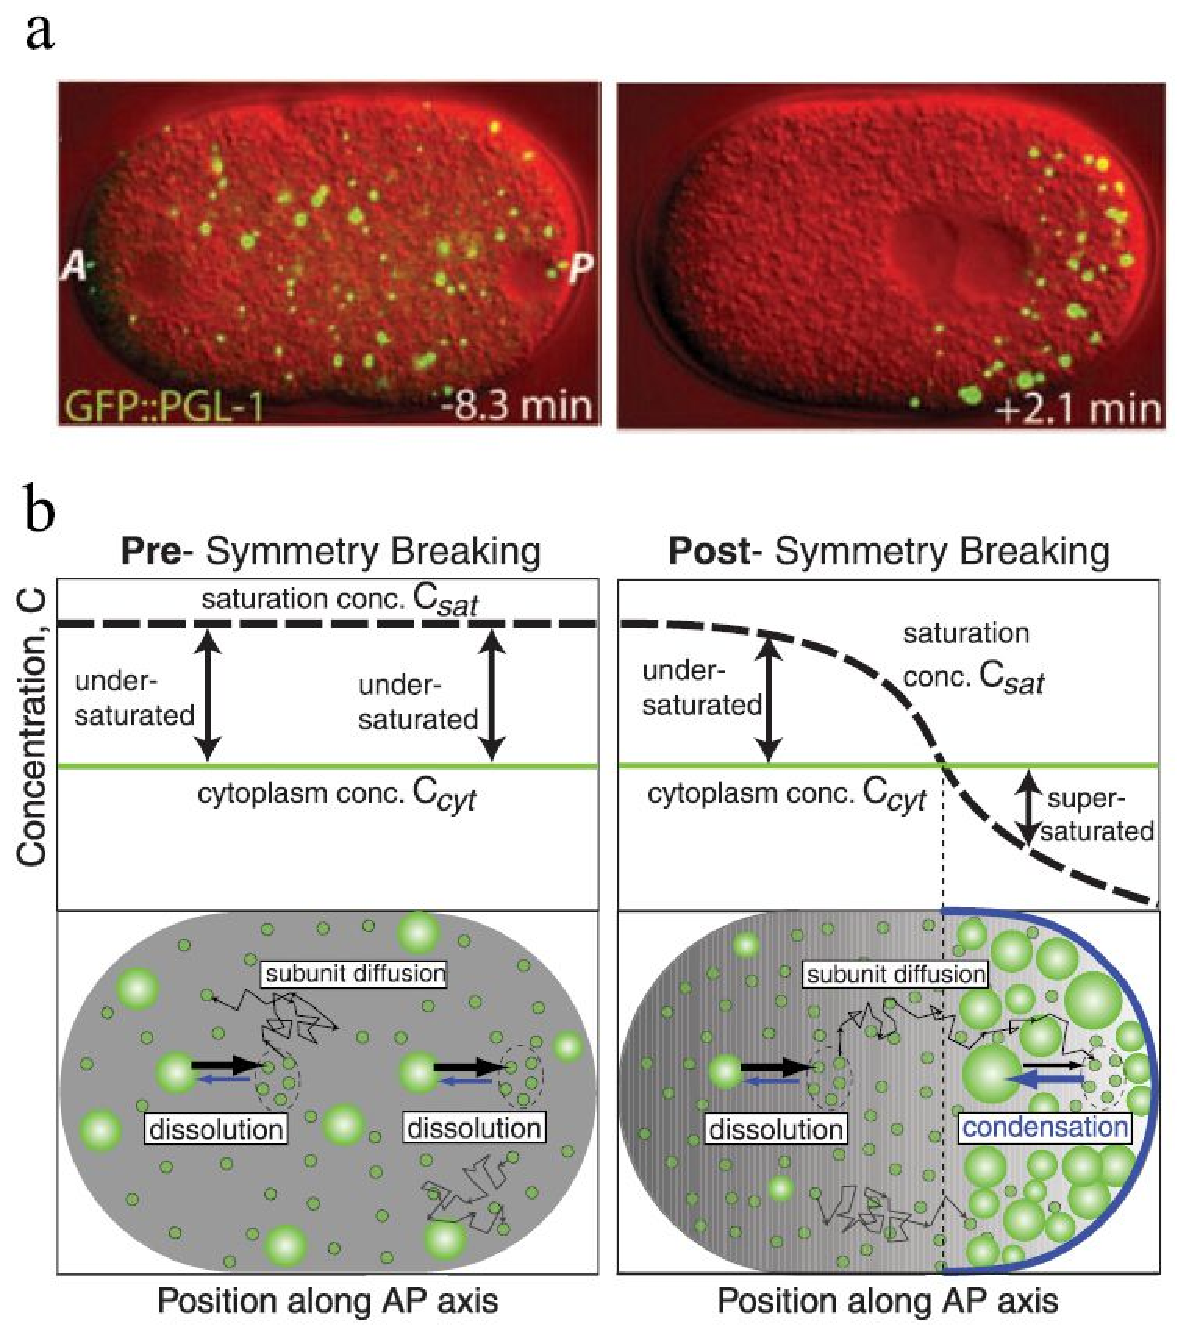
\includegraphics[scale=0.5]{MainContent/BioFigures/gradient.pdf}
\caption{\textbf{Segregation of P granules in early \textit{C. elegans} embryo.}
(A) Initially well mixed P granules (in green) migrate from the anterior to the posterior side of the cell, prior to the first cell division.
Time measured relative to the meeting of two pro-nuclei.
(B) Spatially dependant saturation concentration is established along the anterior-posterior axis, leading to droplet growth on the posterior side and dissolution events on the anterior side. 
Reprinted from Berry et al. \cite{Berry2018} and slightly modified with permission from the publisher with License number 1210876-1.
}
\label{fig:gradient_change}
\end{figure}

Furthermore, it was also shown that the primary mechanism behind localization of P granules was a spatially dependant demixing concentration along the anterior-posterior axis; see \figref{fig:gradient_change}B.
This led to formation and growth of the granules at the posterior side and dissolution events at the anterior side.
Consequently, localization of P granules was anti-correlated with the MEX-5 gradient.

\subsection{Chemical reactions}

After phase separation induces the formation of biomolecular condensates, the cell now has to actively tune condensate properties, so they do not coalesce and clump into one single aggregate.
It is very likely that cells utilize active processes to regulate the function and structure of these condensates, such as: a) Utilizing molecular chaperones and b) Enzymes that facilitate post translational modifications (PTMs) of proteins.
We will mainly focus on these two broad sub-types of active processes in this chapter and discuss them next. 

\subsubsection{Molecular chaperones}

Molecular chaperones are proteins which convert energy into reformulating protein-protein interactions; see Refs. \cite{Akerfelt2010,Tyedmers2010}, and are known to control dynamics, structural properties (for example, increasing porosity of condensates to enhance material exchanges) and stability of stress granules when inducing and removing stress.

Jain et al. \cite{JAIN2016487} investigated in vivo the structural properties of stress granules (which encompass a dynamic shell with a stable core; see \figref{fig:architecture}).
Interactions of the core and the shell (and thus the stability of stress granules) were shown to be modulated by a chaperone TRiC/CCT, which also was identified as a key component of stress granules.
Similarly, Mateju et al. \cite{Mateju2017} identified the role of chaperones named HSP70 in preventing the formation of aberrant stress granules (containing misfolded proteins), which are thought to be the key culprits in diseases such as amyotrophic lateral sclerosis (ALS) in human cells.
Furthermore, HSP70 also aides the dissolution of these stress granules when stress is removed; also see Ref. \cite{Wallace2015}, thereby showing that chaperones can act as quality control managers to prevent aggregation of misfolded proteins, and preserving the dynamics of stress granules. 

Additionally, Qamar et al. \cite{QAMAR2018720} showed that a chaperone called transportin regulates FUS (FUused in Sarcoma - an RNA binding protein) condensation and phase separation in neuron terminals; see Ref. \cite{Chen2019}, and is important for preventing diseases such as familial amyotrophic lateral sclerosis (fALS) and frontotemporal lobar degeneration (FTLD).

\subsubsection{Post-Translational Modifications of proteins}

PTMs of proteins are also considered as a key regulating mechanism of the dynamics and structure of condensates, which function by adding key functional groups to proteins, thus modifying their interactions with other biomolecules.

Hofweber et al. \cite{Hofweber2019} investigated the role of PTMs of RBPs (RNA-binding proteins) in regulating the dynamics of Ribonucleoprotein (RNP) granules, which are condensates consisting of RBPs and RNA.
Weak interactions between RBPs and RNA are responsible for phase separation, which are reduced by slow Arginine methylation (a type of PTM) of RBPs, thereby almost always inhibiting phase separation; see Refs. \cite{QAMAR2018720,Ryan2018,NOTT2015936}.
Arginine methylation of RBPs is thought to regulate RNP granules by two methods - through modifications of protein-protein/RNA interactions and through altering the composition of RBPs throughout the cytoplasm or in the nucleus. 
Interestingly, Arginine methylation is found to both suppress; see Refs. \cite{Dolzhanskayaw2006,Tsai2016}, and facilitate; see Refs. \cite{Matsumoto2012,ArribasLayton2016}, the dynamics and formation of RNP granules.

Contrary to Arginine methylation, Phosphorylation (another type of PTM) is known to be a fast and reversible mechanism and is known to both - suppress; see Refs. \cite{Rhoads2018,Wang2018}, and promote; see Refs. \cite{KAMPERS1996344,Vanderweyde8270}, phase separation. 
Similar to Arginine methylation, Phosphorylation seems to be a key mechanism through which the dynamics, formation and dissolution of RNP granules can be tuned.
Phosphorylation is thought to regulate RNP granules through altering the composition of RBPs by promoting or degrading them, thereby controlling RNP granule formation; see Refs. \cite{Sfakianos2018,MAHBOUBI20151725}, and dissolution; see Refs. \cite{Aranda2011,KRISENKO201527803,Reineke2018}. 
Ambadipudi et al. \cite{Ambadipudi2017} and Wegmann et al. \cite{Wegmann2018} found that Tau phosphorylation changes the charge distribution on the microtubule-binding domain of Tau and enhances electrostatic interactions and promotes phase separation and the growth of Tau droplets.
These droplets are precursors to Tau aggregates, accumulation of which play a role in Alzheimer’s disease; see Refs. \cite{Williams2006,Mucke2009}.

Thus, both - Arginine methylation and Phosphorylation in conjunction, can either promote or inhibit phase separation and dynamics of RNP granules, and thus are good candidates for tuning phase separation and dynamics of RNP granules; also see Refs. \cite{Schisa2021,VelazquezCruz2021}.
Lastly, Glycosylation is another PTM which regulates phase separation. 
In particular, Roth et al. \cite{Roth2017} found for the first time an inverse correlation between Phosphorylation and O-GlcNAcylation in human colon cells in regulating phase separation and inhibiting tau protein condensation. 

Enzymatic reactions can also play a role in the dynamics of condensates. 
In particular Hondele et al. \cite{Hondele2019} found that DEAD-box ATPase family can control formation and dissolution dynamics of RNA condensates in both - prokaryotes and eukaryotes.
They showed that ATPase exists in an ATP-bound state, which promotes phase separation of condensates, and an ATP free state, which accentuates condensate dissolution. 
Utilizing chemical reactions to control droplet growth has also been reviewed recently by S\"{o}ding et al. \cite{SODING20204}, where the authors put forward two important mechanisms - Enrichment inhibition; see Refs. \cite{Wang2014,Kirschbaum2021}, and Localization induction; see Refs. \cite{Langelier2012,Kirschbaum2021}.

These examples clearly highlight that chemical reactions play an important role in tuning the dynamics and stability of condensates. 

\subsection{Regulation of pH and temperature}

pH as a regulatory mechanism for phase separation inside the cell has been studied extensively; see Refs. \cite{Orij2011,Kroschwald2018,Peters2013,Petrovska2014}.
In particular, Bizzari et al. \cite{Bizzarri2008} and Orij et al. \cite{Orij2011} were one of the first to focus on pH as a regulatory mechanism for the cell. 
Orij et al. \cite{Orij2011} focused the yeast species \textit{Saccharomyces cerevisiae} and demonstrated pH as a fast and simple mechanism which the cell uses to spatially organize it's intracellular condensates.

Munder et al. \cite{Munder2016} in their seminal work, investigated how eukaryotic cells (budding yeast) regulate pH in their cytoplasm to control the mobility and structual properties of the condensates.
In their natural habitat, yeast cells typically live in acidic environments (pH $\approx 5.5$), but the cytoplasm is kept at a neutral pH in normal circumstances (pH $\approx 7.3$).
However, when faced with nutrition scarcity,
Munder et al. observed that upon acidification, the cytoplasm transitions reversibly from liquid-like to gel-like structure; see \figref{fig:pH_change}.
\begin{figure}[tb]
\centering
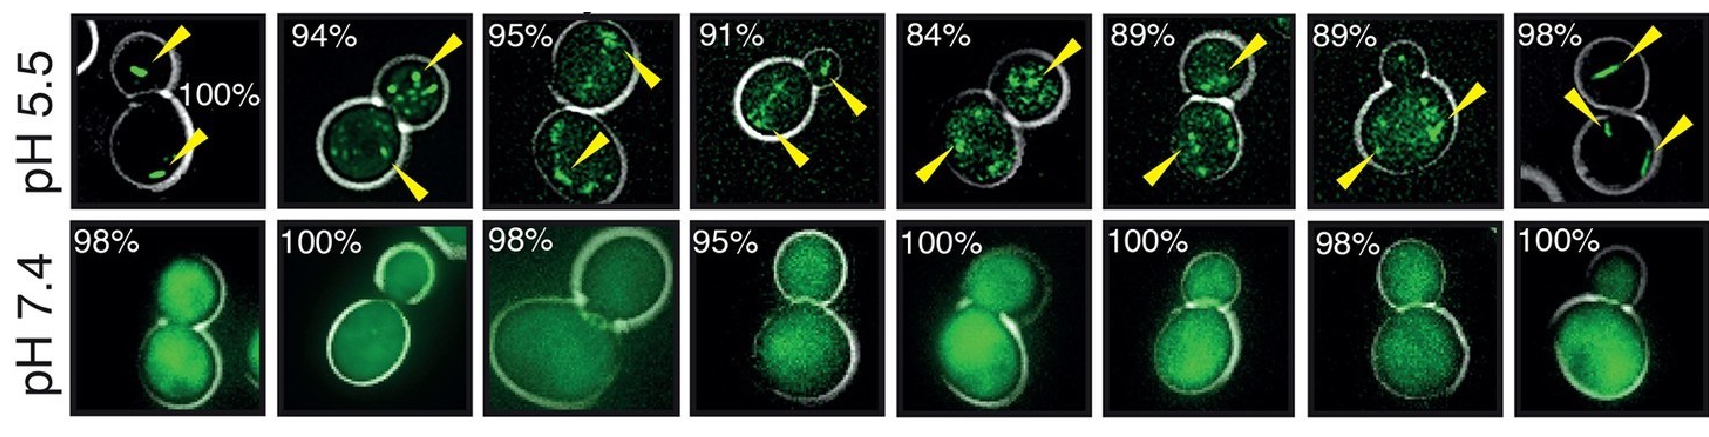
\includegraphics[scale=0.53]{MainContent/BioFigures/ph_change.pdf}
\caption{\textbf{Acidification of cytoplasm induces aggregation of proteins into structures.}
Proteins aggregate into structures depending on cytosolic pH.
When pH is lowered from 7.4 (middle row) to 5.5 (top row), proteins assemble into structures (green dots, top row) and help the transition of the cytoplasm from a liquid-like to a gel-like entity.
These structures were absent and proteins are well mixed when the cytoplasm was almost pH neutral (bottom row), but present when the cytoplasm becomes acidic (top row).
Reprinted with permission from Munder et al. \cite{Munder2016} and slightly modified under the Creative Commons Attribution License.
}
\label{fig:pH_change}
\end{figure}
The transition, which is facilitated through many proteins forming peculiar structures upon a change in cytosolic acidity, is functionally important, as when the cytoplasm is not allowed to solidify, the yeast cells simply die.

Organisms can also regulate phase separation utilizing temperature as a control parameter.
For example, the effect of cyclical variations in temperature on the dissolution and reformation of P-granules in early embryos of the \textit{C. elegans} worm was studied by Fritsch et al. \cite{Fritsch2021}, in agreement with earlier works by Putnam et al. \cite{Putnam2019} and \cite{Andresphdthesis2016}, who investigated mixing and de-mixing of P-granules from the cytoplasm.
Fritsch et al. \cite{Fritsch2021} demonstrated through constructing in vivo phase diagrams that physics of phase separation adequately explains this dynamic process of dissolution and reformation of P-granules, which is dictated by local thermodynamic equilibrium.
The P-granules undergo dissolution upon increasing the temperature and their reformation is recovered upon cooling, thus showing that temperature can be a control mechanism that the organism uses to control stability and dynamics of the condensates.

% \figref{fig:temperature_change}A shows the schematic of an early stage embryo of the \textit{C. elegans} worm and the zoomed in view of the embryo studied. 
% As seen from \figref{fig:temperature_change}B, 

Temperature as a control parameter also appears in plants, for example, Zhu et al. \cite{Zhu2022} investigated the link between stress tolerance, temperature and phase separation in \textit{Arabidopsis thaliana} (a model organism in plant based studies) and showed in vivo that RNA-binding proteins called RBGD2 and RBGD4 condense upon increase in temperature, thus improving heat resistance.
Apart from these thermodynamic properties, physical properties of the intracellular environment can also influence condensates, which we discuss next. 
% \begin{figure}[tb]
% \centering
% \includegraphics[scale=0.65]{MainContent/BioFigures/temperature.pdf}
% \caption{\textbf{Effect of temperature on dissolution and formation of P-granules.}
% (A) shows a schematic of an early stage embryo of the \textit{C. elegans} worm and the zoomed in view of the embryo studied with P-granules in yellow. 
% (B) shows P-granules (yellow green dots) undergo cyclical dissolution and reformation subjected to alternating temperatures. 
% Image taken from Fritsch Anatol W., Diaz-Delgadillo Andrés F., Adame-Arana Omar, Hoege Carsten, Mittasch Matthäus, Kreysing Moritz, … Weber Christoph A. (2021). Local thermodynamics govern formation and dissolution of Caenorhabditis elegans P granule condensates. Proceedings of the National Academy of Sciences, 118(37), e2102772118. doi:10.1073/pnas.2102772118.
% }
% \label{fig:temperature_change}
% \end{figure}

\subsection{Physical modifications of intracellular environment}

Inside the crowded environment of the cell; see Ref. \cite{Andre2020}, dynamics of biomolecular condensates are coupled with the dynamical properties of the cytoskeletal filaments, and can thus influence each other's size, shape and structural properties; see \figref{fig:mechanical_forces_in_cells}.
We will discuss some important studies which highlight how the cytoskeletal networks affects the spatiotemporal dynamics of condensates. 

\begin{figure}[tb]
\centering
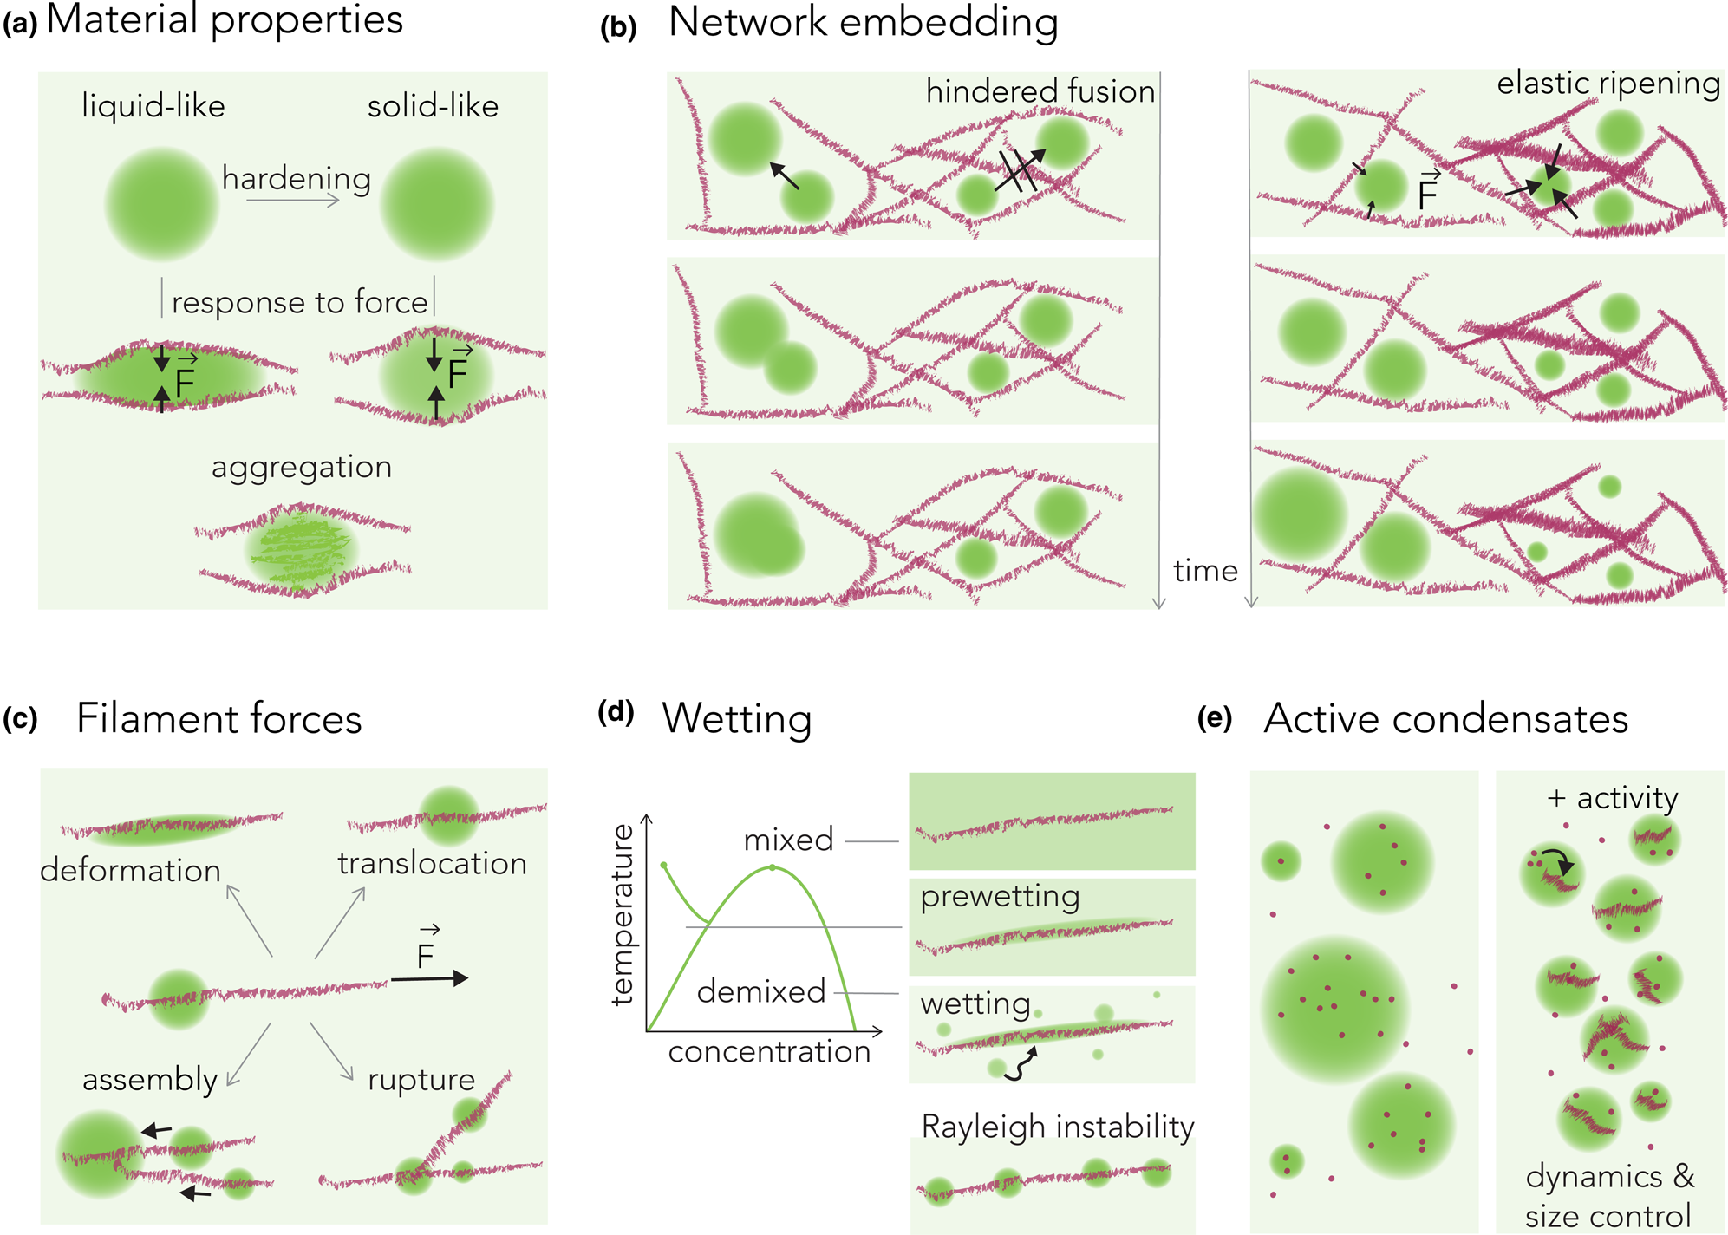
\includegraphics[scale=0.53]{MainContent/BioFigures/scaffolds.pdf}
\caption{\textbf{Cytoskeletal networks influence the stability and dynamics of condensates.}
(A) Cytoskeletal filaments influence condensate stability by exerting physical forces; see Ref. \cite{Enos2018}.
(B) Cytoskeletal networks can stabilize large condensates through mechanical forces and act as a `condensate sieve';  see Ref. \cite{Quiroz2020}.
Heterogenous elastic networks can reverse \textit{Ostwald-Ripening} and stabilize small droplets; see Refs. \cite{Rosowski2020,D0SM00628A}.
(C) Contracting or extending networks can control droplet dynamics; see Ref. \cite{Enos2018}.
(D) Wetting phenomena can also influence and drive phase separation; see Ref. \cite{Setru2021}.
(E) Active processes can stabilize emulsions of many droplets; see Refs. \cite{Zwicker2015,Review2019}.
Reprinted from Wiegand et al. \cite{Wiegand2020} with permission from the publisher with License number 1210880-1.
}
\label{fig:mechanical_forces_in_cells}
\end{figure}

Feric et al. \cite{Feric2013} in their pioneering work investigated the role of nuclear actin in Oocytes of the frog \textit{Xenopus laevis}.
They demonstrated the importance of actin mesh in keeping the typically large nucleoli ($\sim 450 \, \mathrm{\mu m}$ in diameter) from coalescing and sedimenting under gravity, thus demonstrating the mechanically stablizing role of actin.
Furthermore actin network also acts as a `condensate sieve', allowing smaller condensates to diffuse while arresting the dynamics of bigger condensates.

Similarly, Enos et al. \cite{Enos2018} showed that Pericentriolar material (PCM - outer layer of centrosomes) dissolution in \textit{C. elegans} embryo is governed by a dephosphorylation process of the scaffolding protein known as SPD-5 and physical pulling forces ripping apart the SPD-5 scaffolding; similar to the schematics in \figref{fig:mechanical_forces_in_cells}A.  More recently, Garcia Quiroz et al. \cite{Quiroz2020} have shown that keratin filament networks in mammalian skin cell layers can stabilize condensates known as keratohyalin granules; see \figref{fig:mechanical_forces_in_cells}B, and keep them from fusing by caging, thus keeping individual condensates apart from each other and maintaining their stability.

B\"{o}ddekker et al. \cite{Boeddeker2022} investigated the interaction between cytoskeletal filaments (microtubules) and condensates (stress granules) to understand the role of viscoelastic environments in controlling phase separation inside U2OS epithelial cells.
In the vicinity of stress granules, microtubule network density is higher and the network is severely deformed.
Polymerization and depolymerization of the microtubules directly affected the surface properties of stress granules, which hints at tuning of networks as a control mechanism for the cell.

The presence of heterogeneous elastic networks can also affect phase separation - in particular, reverse \textit{Ostwald-Ripening} - where large droplets give up material and feed the smaller droplets, as shown by Rosowski et al. \cite{Rosowski2020,D0SM00628A} and Vidal-Henriquez et al. \cite{VidalHenriquez2021}, shedding light on potentially controlling ripening processes by taking advantage of heterogeneous elastic networks inside cells.
There also have been exciting recent advances in exploring the viscoelastic network of chromatin, which exhibits slow coarsening of condensates and retards coalescence.
In particular, Qi et al. \cite{Qi2021} studied condensate coalescence in the presence of chromatin networks using theory and simulations and showed that condensate (nucleoli) - chromatin interactions promoted nucleation, but hindered coalescence.
Similarly, anomalous diffusion of condensates due to physical constraints from the viscoelastic chromatin network was reported by Lee et al. \cite{Lee2021}, where the coarsening exponent was found to be $\beta \sim 0.12$, as opposed to the theoretical prediction of $\beta = 0.33$; see Refs. \cite{Review2019,Weber2017}.

Lastly, wetting phenomena is also responsible to driving phase separation, for example, Jiang et al. \cite{Jiang2015} showed that a protein called BuGZ forms liquid droplets on microtubules.
Similarly, Setru et al. \cite{Setru2021} investigated the dynamics of droplets formed by condensation of a protein called TPX2 on microtubules; see \figref{fig:mechanical_forces_in_cells}D. 
They showed that a fluid instability drives the condensation and TPX2 droplets not only form a one dimensional lattice on the microtubule branch, but the inter-droplet distance increases with increasing TPX2 concentration.
Taken together, all the above examples show the interplay between condensate dynamics and the intracellular environment. 
However, instead of controlling the properties of it's internal environment, the cell can also regulate properties of the condensates themselves, which we discuss next. 

\subsection{Modifying properties of condensates}

Recently, applications from pharmaceutical and food industries, such as the usage of `Pickering agents' in stabilizing emulsions; see review by Yang et al. \cite{Yang2017} and references therein, have inspired similar studies in the context of biological cells.

Pickering agents are solid particles, typically nanoscale sized, which adsorb on the interfaces of liquid droplets with partial wetting. Adsorption is favoured energetically, thereby reducing the affinity of the droplets towards lowering their surface area, leading to slowing down of their coarsening.
The discuss a few studies which suggest that cells may recruit biopolymers (which are plenty in the cytoplasm; see Ref. \cite{Burla2019}), as Pickering agents.
This is exciting as it could provide an additional pathway for the cell to as an organizing principle for intracellular biomolecular condensates.

Folkmann et al. \cite{Folkmann2021} studied and investigated mechanisms responsible for anomalous coarsening of P granules (which are made up of RNA and a protein called PGL-3) in \textit{C. elegans} when transitioning from egg to embryo.
Earlier studies by Putnam et al. \cite{Putnam2019} have shown that an intrinsically disordered protein called MEG-3 stabilizes PGL-3 droplets by forming a scaffold around them, thus spatially regulating their condensation in the cytoplasm.
Folkmann et al. then identified MEG-3 clusters as a Pickering agents inside the cell, which adsorb to the interface of P granules and pose as a physical obstacle, slowing down their coarsening.

Similarly, Zhang et al. \cite{Zhang2018} suggested that EPG-2 clusters act in a similar way as MEG-3 to regulate the dynamics of PGL droplets.
EPG-2 accelerates the transition of PGL-1/3 droplets into gel-like structures, rendering them less dynamic and more stable.
Lastly, Tauber et al. \cite{Tauber2020} also suggested a similar adsorption mechanism, indicating that mRNAs aggregating on the surface of protein condensates may act as stabilizing agents.

All the above examples clearly exhibit the complex coupling between the condensate dynamics and dense networks, suggesting cells can tune the network properties in their interior to exert spatiotemporal control over formation, stability and dynamics of the condensates. 

Computational and theoretical models can help unravel the coupling of condensates and the intracellular environment and mechanisms of spatiotemporal control by the cell.
Computational models are generally useful, as exploring large parameter spaces is not a limitation, relative to experimental studies.
Additionally, studying the effects of control parameters on long time and length-scales is an advantage for computational models.
We next discuss some computational and theoretical approaches used to study phase separation behaviour.

\section{Modelling and simulations of phase separation}

Broadly speaking, computational models fall in two main categories: \textit{Field-based} models and \textit{Particle-based} models.

\subsection{Field-based models}

The field-based models typically have a continuum based approach, where the presence and effects of various biomolecules is represented by changes in the field variables like density or composition $\phi(\vec{x})$.
Then, a general free energy of the system is formulated as a functional of the composition $F[\phi(\vec{x})]$ with an aim of minimizing the free energy, subject to problem specific constraints, using numerical or analytical approaches.
Typically, phase separation will occur when a generic composition field will minimize the free energy functional $F$.
Additionally, such free energy formulations can then be extended to include the effects of multi-component fluids, chemical reactions, fluid flows and model phase separation in polymers as well.

One such field-based model has been typically used to model phase separation; namely the \textit{Cahn-Hilliard} model; see Ref. \cite{CahnHilliardEq}.
For example, the \textit{Cahn-Hilliard} model, along with theoretical models, has been utilized and modified to study phase separation in binary and ternary mixtures.
In particular, Berry et al. \cite{Berry2015} investigated the disassembly and assembly of nucleoli and ENDs (extranucleolar droplets) in \textit{C. elegans} embryos using a modified \textit{Flory-Huggins} theory; see Ref. \cite{FloryBook} for ternary solutions.
Gasior et al. \cite{Gasior2019} used a multi-phase \textit{Cahn-Hilliard} model to study binding and unbinding of different RNA-protein complexes with an aim to understand spatial patterning and it's role in intracellular organization.

The \textit{Cahn-Hilliard} model has also been used to study phase separation in multi-component systems and used to uncover different morphologies and coarsening behaviour by Mao et al. \cite{Mao2019}.
Similarly, Vweza et al. \cite{ijms22136675} investigated the effects of macromolecular crowding on the coarsening dynamics and morphologies of small condensates, shedding light on their growth and stability.
Field-based models have also found applications in the area of polymer phase separation.
In particular, phase separation in block copolymers has been studied by Ren et al. \cite{Ren2001} and by Fredrickson et al. \cite{Fredrickson2002}, where they recovered various morphological structures (cylindrical, lamellar) by using a modified version of the \textit{Cahn-Hilliard-Cook} model.

Field-based models have also been successful in studying effects on long time and length-scales.
In particular, Weber et al. \cite{Review2019,Weber2017} have demonstrated coarsening behaviour and effects of chemical gradients on phase separation. 
Jacobs et al. \cite{Jacobs2021,JACOBS2017683}
studied phase separation in multi-component mixtures and the effect of random interactions in the stability of multiple phases.  
The effects of chemical reactions and elasticity have been simulated using field-based models as well.
For example, Vidal-Henriquez et al. \cite{VidalHenriquez2021} have studied and modelled the effects of elasticity of chromatin network on droplets, which can serve as a base for further theoretical investigations.
Lastly, the effects of chemical reactions on droplet sizes, stability and coarsening behaviour in ternary mixtures was studied by Wurtz et al. \cite{Wurtz2018}.

Taken together, we have summarized a few representative examples where field-based models have been used to investigate phase separation in diverse areas. 
However, these models have restricted application pertaining to phase separation in the cell, as they do not possess the granularity, specificity and the resolution needed to consider specific protein-protein interactions, as the internal composition of the cytoplasm in the cell is composed of hundreds of biomolecules with specific sequences; see Ref. \cite{Burla2019}.
In the following section, we will elaborate on a different type of model, which alleviates some of the drawbacks of the field-based models. 

\subsection{Particle-based models}

Where Field-based models lack, Particle-based models try to fill that void.
Particle-based models essentially aim to represent different phases in a phase separating mixture as an ensemble of particles.
These particles are typically governed by force fields, which takes into account various interactions arising from chemical bonds and long range interactions such as Coulomb interactions.
A significant advantage particle-based models have over field-based models is the ability to take into account correlations across atoms or molecules without being explicitly integrated in the method.
These models are often used in conjunction with experiments and are typically used to extract features and information about phase separation at a molecular level.

Particle-based models fall into different categories as well, some being \textit{Molecular dynamics} simulations, \textit{Coarse-grained} models and \textit{Lattice-based} models.
Although these models overlap quite a bit in their formulation and distinction between them is not always clear, we will consider them separately and elaborate on each of their merits and demerits. 

\subsubsection{Molecular dynamics simulations}

Simulations falling under the broad umbrella of \textit{Molecular dynamics} simulations; proposed by Alder et al. \cite{Alder1959}, typically evolve dynamics of particles in time using numerical integration of Newton's laws of motion.
For example, Chu et al. \cite{Chu2021} investigated the temperature and charge pattern dependence of a chaperone protein called Swc5 on phase separation in biomolecules and role of Swc5 in chromatin formation.
On similar lines, Farr et al. \cite{Farr2021} studied effects of chromatin compaction on nucleosome dynamics.

To study the interplay between long and short range interactions of intrinsically disordered proteins on the stability, structure and dynamics of condensates, Hazra et al. \cite{Hazra2021} used a coarse-grained molecular dynamics simulation model.
A similar model was also utilized by Espinosa et al. \cite{Espinosa2020} to uncover physical principles governing the stability of multi-component condensates and the effects of networks on these condensates.

However, considering that the crowded environment of the biological cell and the presence of hundreds of biomolecules; see Ref. \cite{Ellis2003}, Molecular-dynamics simulations are extremely expensive, and the computational costs scale up quickly when simulating biomolecules on the level of a single atom or molecule in three dimensions.
Furthermore, these simulations lack an important feature, which is relevant in the case of biomolecules - which is their inability to predict rare events like conformational changes in proteins, protein folding and nucleation events like the initial formation of nucleolus; see Ref. \cite{Falahati2016}.
Some of these drawbacks can be eliminated by using \textit{Coarse-grained} models, which we will discuss next. 
\subsubsection{Coarse-grained models}

\textit{Coarse-grained} models partially alleviate the computational expensiveness of Molecular dynamics simulations.
They consider ensembles or clusters of atoms which are averages over length scales and timescales, thus effectively reducing computational costs.
In the context of biomolecules, this can be thought of as a single interacting element which represents a particular group of atoms.
These models have often been used in conjunction with experiments to uncover mechanisms of spatiotemporal control of the cell over the formation and features of it's condensates.

For example, Kaur et al. \cite{Kaur2021} employed a coarse-grained model of a ternary system consisting of peptides and RNA complexes to demonstrate the importance of mixture compositions in the spatial organization of multi-component condensates. 
Similarly, Tejedor et al. \cite{Tejedor2021} utilized a similar model to study impact of RNA on condensate transport, stability and spatiotemporal control over condensate dissolution and formation.

Recently, Benayed et al. \cite{Benayad2021} used a modified version of MARTINI coarse-grained model; see Refs. \cite{deJong2013, Marrink2007}, to study biopolymer phase separation in the context of droplet formation of the disordered protein called FUS-LCD.
Zhang et al. \cite{Zhang2021} utilized a coarse grained approach to disentangle the roles of valency, stoichiometry and binding strength of phase separating two-polymer systems; shedding light on how the cell might be able to tune these roles via chemical modifications or synthesis/degradation to alter and control the properties of the condensates. 

\subsubsection{Lattice-based models}

\textit{Lattice-based} models have also been utilized to study the physics of phase separation; for example, the phenomena of gelation in phase separation in ternary systems and the effects of intrinsically disordered linkers on droplet formation by Harmon et al. \cite{Harmon_2018, Harmon1}.
Similarly, Ruff et al. \cite{Ruff2021} explored the role of scaffolds (which are multi-valent macromolecules) in the assembly and disassembly of condensates. 
Notably, a recent open-source package named LASSI (LAttice simulation engine for Sticker and Spacer Interactions) has been developed by Choi et al. \cite{LASSI} to study phase separation in multi-component systems; see Refs. \cite{Dar2020,Ranganathan2020}.

In this thesis, we focus on studying and capturing the effects of chemical reactions and external chemical gradients on phase separated droplets at a cellular scale, we will use field-based modelling and not particle-based approaches. 
This method allows us to disentangle and simulate them separately, especially on long time and length-scales.

\section{Outline of the thesis}

In this thesis, we will develop a fast and efficient numerical model for simulating dynamics of droplets, which are phase separated from a dilute phase, without solving the computationally expensive \textit{Cahn-Hilliard} equation describing phase separation.
Our motivation comes from biology, where biomolecular condensates (which are formed in the intracellular environment) are spatiotemporally controlled by the cell using various mechanisms to ensure proper functioning and survival of the cell.
Out of many such control mechanisms, the cell uses chemical reactions and external chemical gradients to maintain control over the dynamics, structure and size of these condensates.
In this thesis, we will utilize our numerical model to disentangle and study the effects of chemical reactions and external chemical gradients on the dynamics of droplets. 

We start by introducing basic thermodynamic principles, leading upto dynamics of phase separation, in Chapter \ref{chap:Chapter_2}.
We then discuss an analytical approximation of the \textit{Cahn-Hilliard} model, i.e. the continuous model for phase separation, which describes dynamics of phase separated droplets.
In Chapter \ref{chap:Chapter_3}, we will build upon this analytical approximation to formulate an effective droplet model, in which we separately consider the dynamics of droplets and the dilute phase.
We assume that droplets co-exist with a background phase, described by a discretized volume fraction field, and we study their interaction with the background phase by discretizing their vicinity.
The growth and drift dynamics of droplets follow from the material fluxes exchanged between the droplet and the background phase.
These fluxes also affect the dynamics of the dilute phase itself, which we describe via reaction-diffusion equations, thus making our effective droplet model orders of magnitude faster than the \textit{Cahn-Hilliard} model.

In Chapter \ref{chap:Chapter_4}, we use a synthetic test-case to study the effects of simulation parameters of the effective droplet model and find their optimum values by comparing with the ground truth, i.e. simulations using the the \textit{Cahn-Hilliard} model.
In Chapter \ref{chap:Chapter_5} we use the optimum parameters obtained from Chapter \ref{chap:Chapter_4} and validate the effective droplet model with known literature.
We simulate various scenarios ranging from single droplet in presence of chemical reactions and external chemical gradients to mean-field coarsening of $10^5$ droplets in a large dilute emulsion and compare these with simulations using the the \textit{Cahn-Hilliard} model (wherever computationally viable) and analytical predictions.
We demonstrate that the effective droplet model is able to accurately capture droplet dynamics across diverse situations in and we are able to disentangle and separately study the effects of chemical reactions and external chemical gradients on droplet growth and drift.
We find that the effective droplet model is a viable and a pragmatic option for fast and computationally efficient simulations of phase separated droplets in large many-droplet emulsions.
Finally, in Chapter \ref{chap:Chapter_6} we discuss future improvements and extensions to the effective droplet model.



